\documentclass{standalone}
\usepackage{graphicx}	
\usepackage{amssymb, amsmath, amsthm}
\usepackage{color}

\usepackage{tikz}
\usetikzlibrary{math, calc, arrows.meta}

\definecolor{light}{RGB}{220, 188, 188}
\definecolor{mid}{RGB}{185, 124, 124}
\definecolor{dark}{RGB}{143, 39, 39}
\definecolor{highlight}{RGB}{180, 31, 180}
\definecolor{gray10}{gray}{0.1}
\definecolor{gray20}{gray}{0.2}
\definecolor{gray30}{gray}{0.3}
\definecolor{gray40}{gray}{0.4}
\definecolor{gray60}{gray}{0.6}
\definecolor{gray70}{gray}{0.7}
\definecolor{gray80}{gray}{0.8}
\definecolor{gray90}{gray}{0.9}
\definecolor{gray95}{gray}{0.95}


\begin{document}

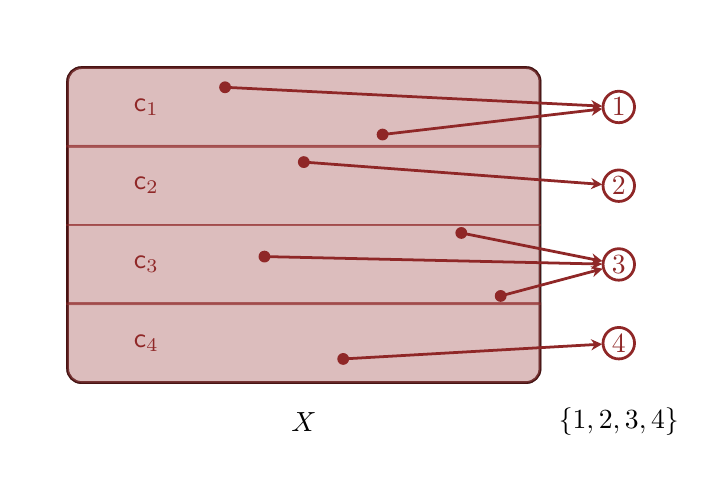
\begin{tikzpicture}[scale=1]
  \draw[white] (-0.5, -1) rectangle (8, 4.5);
  \draw[rounded corners=5, color=black, line width=1] (0, 0) rectangle (6, 4);
  \node at (3, -0.5) { $X$ };
  
  \filldraw[draw=dark, fill=mid, opacity=0.5, line width=1]
    (0, 3) -- (6, 3) {[rounded corners=5] -- (6, 4) -- (0, 4)} -- cycle;
  \node[dark] at (1, 3.5) { $\mathsf{c}_{1}$ };

  \filldraw[draw=dark, fill=mid, opacity=0.5, line width=1]
    (0, 2) -- (6, 2) -- (6, 3) -- (0, 3) -- cycle;
  \node[dark] at (1, 2.5) { $\mathsf{c}_{2}$ };
    
  \filldraw[draw=dark, fill=mid, opacity=0.5, line width=1]
    (0, 1) -- (6, 1) -- (6, 2) -- (0, 2) -- cycle;
  \node[dark] at (1, 1.5) { $\mathsf{c}_{3}$ };
        
  \filldraw[draw=dark, fill=mid, opacity=0.5, line width=1]
    (0, 1) -- (6, 1) {[rounded corners=5] -- (6, 0) -- (0, 0)} -- cycle;
  \node[dark] at (1, 0.5) { $\mathsf{c}_{4}$ };

  \foreach \i in {1, 2, 3, 4} {
    \draw[dark, line width=1] (7, 3.5 + 1 - \i) circle (0.2);
    \node[dark] at (7, 3.5 + 1 - \i) { $\i$ };
  }
  \node at (7, -0.5) { $\{1, 2, 3, 4\}$ };
  
  
  \foreach \x/\y/\i in {2/3.75/1, 4/3.15/1, 3/2.8/2, 5/1.9/3, 2.5/1.6/3, 5.5/1.1/3, 3.5/0.3/4} {
    \draw[->, -{Stealth[length=4pt, width=4pt]}, shorten >=6, dark, line width=1] (\x, \y) -- (7, 3.5 + 1 - \i);
    \fill[dark] (\x, \y) circle (0.075);
  }
  

\end{tikzpicture}

\end{document}  